\section{mo\-Impr\-Best\-Fit\-Aspir\-Crit$<$ M $>$ Class Template Reference}
\label{classmo_impr_best_fit_aspir_crit}\index{moImprBestFitAspirCrit@{moImprBestFitAspirCrit}}
One of the possible {\bf mo\-Aspir\-Crit}{\rm (p.\,\pageref{classmo_aspir_crit})}.  


{\tt \#include $<$mo\-Impr\-Best\-Fit\-Aspir\-Crit.h$>$}

Inheritance diagram for mo\-Impr\-Best\-Fit\-Aspir\-Crit$<$ M $>$::\begin{figure}[H]
\begin{center}
\leavevmode
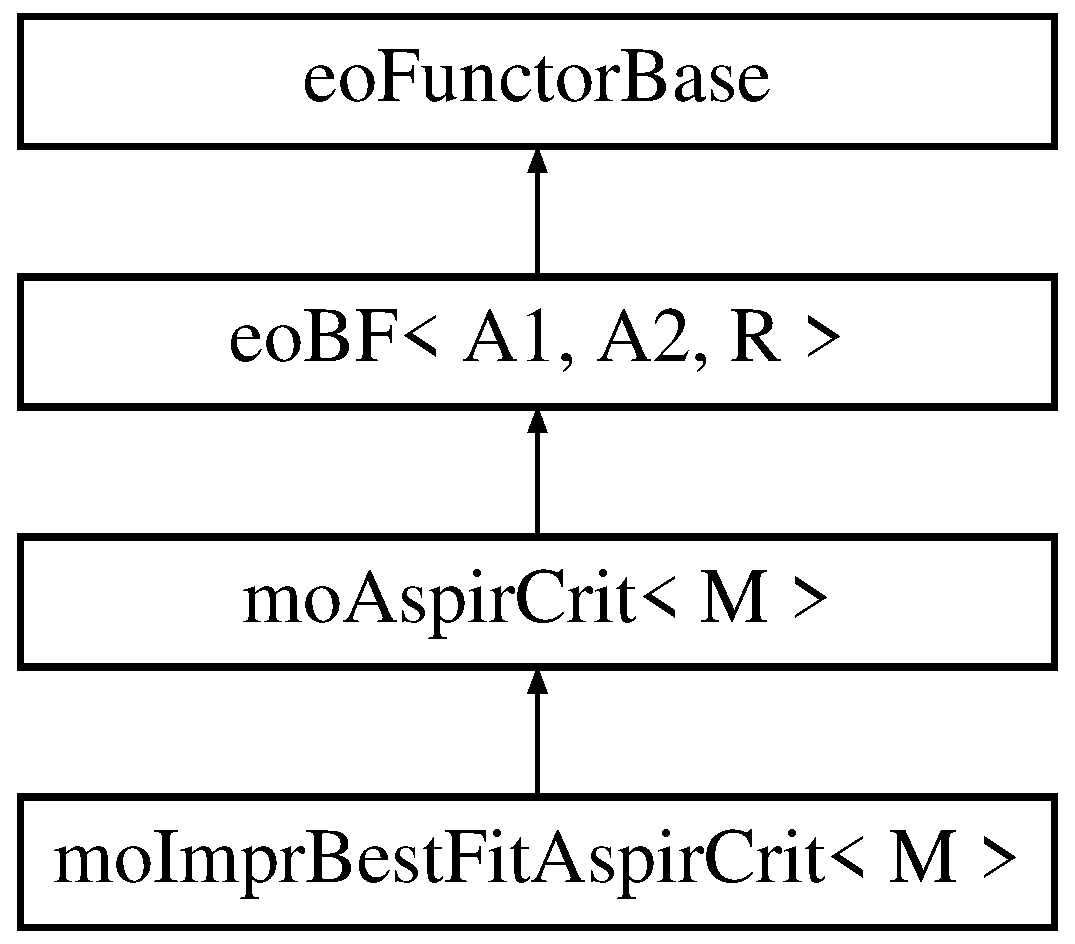
\includegraphics[height=2cm]{classmo_impr_best_fit_aspir_crit}
\end{center}
\end{figure}
\subsection*{Public Types}
\begin{CompactItemize}
\item 
typedef M::EOType::Fitness {\bf Fitness}\label{classmo_impr_best_fit_aspir_crit_0bc1a8c9af99781e662570c04750cca8}

\begin{CompactList}\small\item\em Alias for the fitness. \item\end{CompactList}\end{CompactItemize}
\subsection*{Public Member Functions}
\begin{CompactItemize}
\item 
{\bf mo\-Impr\-Best\-Fit\-Aspir\-Crit} ()\label{classmo_impr_best_fit_aspir_crit_e2c697a5cf3a7696e38bb52b6694a340}

\begin{CompactList}\small\item\em Contructor. \item\end{CompactList}\item 
void {\bf init} ()\label{classmo_impr_best_fit_aspir_crit_ffa451a14ff4ea86fb8bd9fdbc348630}

\begin{CompactList}\small\item\em Initialisation procedure. \item\end{CompactList}\item 
bool {\bf operator()} (const M \&\_\-\_\-move, const {\bf Fitness} \&\_\-\_\-fit)
\begin{CompactList}\small\item\em Function that indicates if the fit is better that the already saved fit. \item\end{CompactList}\end{CompactItemize}
\subsection*{Private Attributes}
\begin{CompactItemize}
\item 
{\bf Fitness} {\bf best\_\-fit}\label{classmo_impr_best_fit_aspir_crit_9e52383f0af8013b4aff0942325e1bf3}

\begin{CompactList}\small\item\em Best fitness found until now. \item\end{CompactList}\item 
bool {\bf first\_\-time}\label{classmo_impr_best_fit_aspir_crit_2d5226c7dd661b33011402dbbbe78265}

\begin{CompactList}\small\item\em Indicates that a fitness has been already saved or not. \item\end{CompactList}\end{CompactItemize}


\subsection{Detailed Description}
\subsubsection*{template$<$class M$>$ class mo\-Impr\-Best\-Fit\-Aspir\-Crit$<$ M $>$}

One of the possible {\bf mo\-Aspir\-Crit}{\rm (p.\,\pageref{classmo_aspir_crit})}. 

This criterion is satisfied when a given fitness is the best ever considered. 



Definition at line 22 of file mo\-Impr\-Best\-Fit\-Aspir\-Crit.h.

\subsection{Member Function Documentation}
\index{moImprBestFitAspirCrit@{mo\-Impr\-Best\-Fit\-Aspir\-Crit}!operator()@{operator()}}
\index{operator()@{operator()}!moImprBestFitAspirCrit@{mo\-Impr\-Best\-Fit\-Aspir\-Crit}}
\subsubsection{\setlength{\rightskip}{0pt plus 5cm}template$<$class M$>$ bool {\bf mo\-Impr\-Best\-Fit\-Aspir\-Crit}$<$ M $>$::operator() (const M \& {\em \_\-\_\-move}, const {\bf Fitness} \& {\em \_\-\_\-fit})\hspace{0.3cm}{\tt  [inline]}}\label{classmo_impr_best_fit_aspir_crit_53f62fb56dcae3051a741f1fddb0204b}


Function that indicates if the fit is better that the already saved fit. 

The first time, the function only saved the current move and fitness.

\begin{Desc}
\item[Parameters:]
\begin{description}
\item[{\em \_\-\_\-move}]a move. \item[{\em \_\-\_\-fit}]a fitnes linked to the move. \end{description}
\end{Desc}
\begin{Desc}
\item[Returns:]TRUE the first time and if \_\-\_\-fit $>$ best\_\-fit, else FALSE. \end{Desc}


Definition at line 52 of file mo\-Impr\-Best\-Fit\-Aspir\-Crit.h.

References mo\-Impr\-Best\-Fit\-Aspir\-Crit$<$ M $>$::best\_\-fit, and mo\-Impr\-Best\-Fit\-Aspir\-Crit$<$ M $>$::first\_\-time.

The documentation for this class was generated from the following file:\begin{CompactItemize}
\item 
mo\-Impr\-Best\-Fit\-Aspir\-Crit.h\end{CompactItemize}
